\chapter*{Instalação e configuração do ambiente}
\label{apendice:1}

\section*{Controlador de versão}

Nesta seção serão apresentado os passos necessários para a criação do repositório utilizado no sistema de controle de versão, junto com a instalação da ferramenta utilizada para trabalhar com este controlador de versão e sua configuração.

Para criar um repositório no Github (ferramenta de controle de versão) utilizado neste trabalho, deve-se acessar a  \textit{url} http://github.com, por meio de um navegador de internet e clicar no botão \textit{"Sign In"}, caso possua conta, caso contrário clique no botão \textit{"Sign up"} e crie sua conta. A Figura~\ref{fig:ap1:pagina_inicial_github} apresenta a página inicial do Github.

\captionsetup[figure]{list=no}
\begin{figure}[h!]
	\centerline{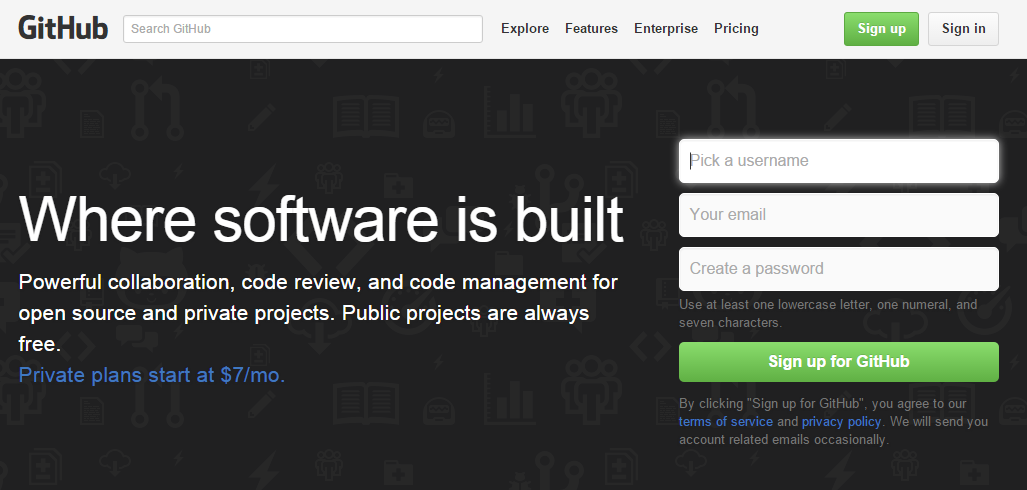
\includegraphics[scale=0.55]{./imagens/apendices/pagina-inicial-github.png}}
	\caption[Página inicial do Github.]
	{Página inicial do Github. \textbf{Fonte:} Elaborado pelos autores.}
	\label{fig:ap1:pagina_inicial_github}
\end{figure}

Para prosseguir no processo de criação do repositório (com a conta já criada), basta clicar no menu \textit{"Sign In"}, realizar o \textit{login} e a página inicial, contendo a lista de seus repositórios será apresentada conforme a Figura~\ref{fig:ap1:pagina_home_github} apresenta.

\newpage
\captionsetup[figure]{list=no}
\begin{figure}[h!]
	\centerline{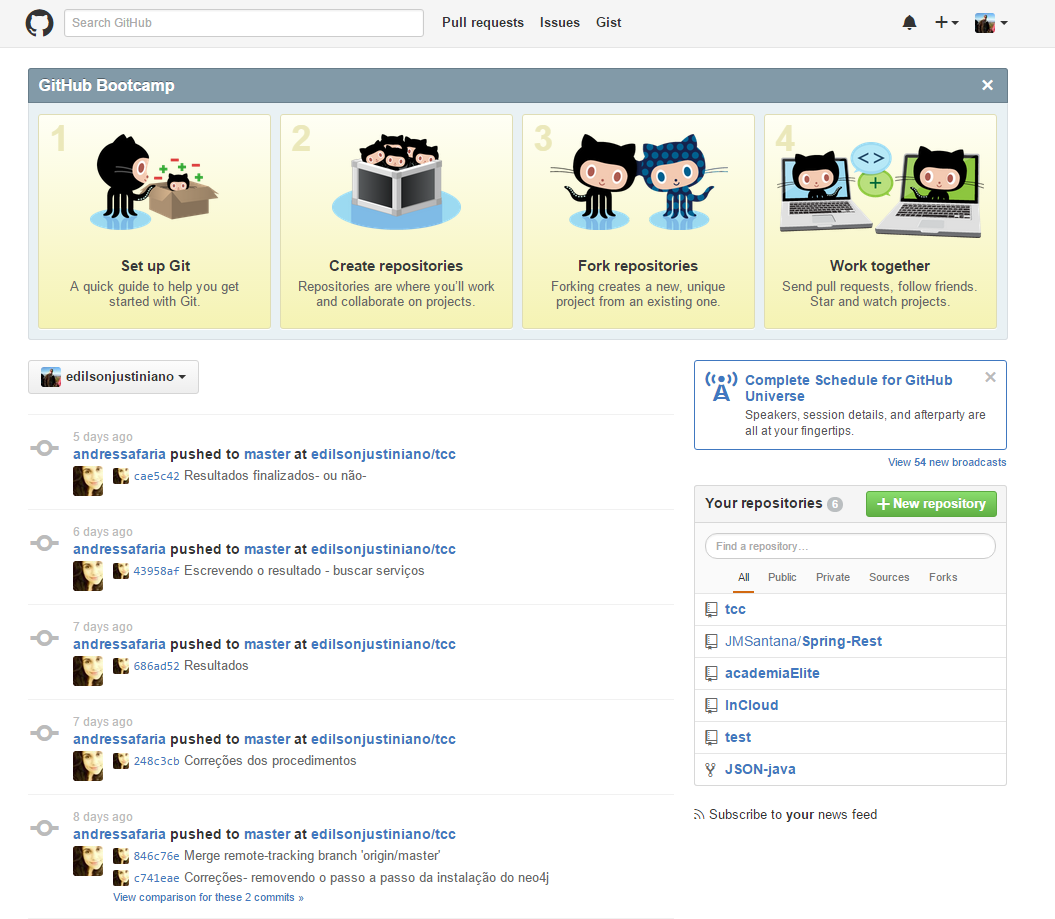
\includegraphics[scale=0.55]{./imagens/apendices/pagina-home-github.png}}
	\caption[Página com a lista de repositórios do usuário no Github.]
	{Página com a lista de repositórios do usuário no Github. \textbf{Fonte:} Elaborado pelos autores.}
	\label{fig:ap1:pagina_home_github}
\end{figure}

 
Nesta seção serão apresentados os passos para a instalação do banco de dados Neo4j.

\par Para realizar o \textit{download} do instalador do banco de dados Neo4j, deve-se acessar a seguinte URL, por meio de um  navegador de internet: http://neo4j.com/download e selecionar a opção desejada. Neste trabalho como já descrito foi utilizada a versão \textit{Community}. A Figura~\ref{fig:download_neo4j} apresenta a página de \textit{download} do Neo4j.

\newpage
\begin{figure}[h!]
	\centerline{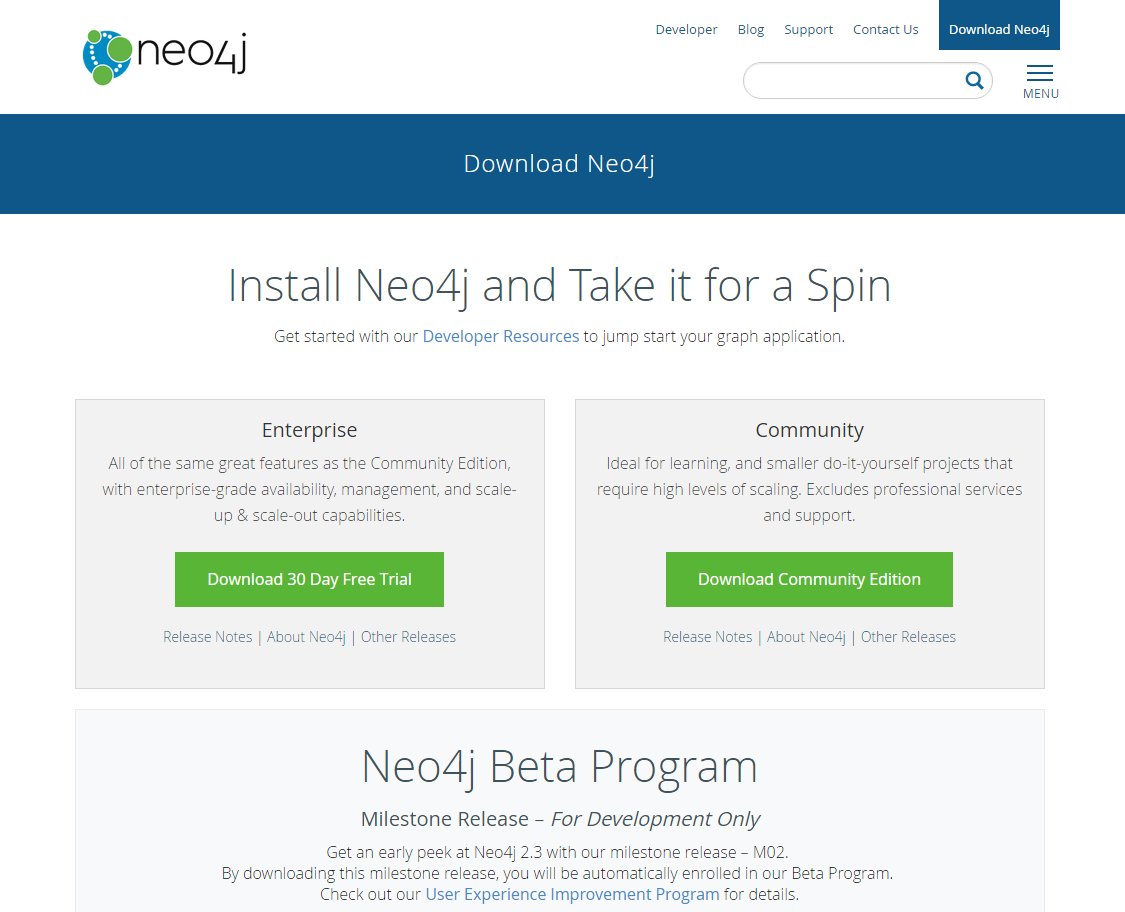
\includegraphics[scale=0.4]{./imagens/download-neo4j.png}}
	\caption[Página de download do Neo4j]
	{Página de download do Neo4j. \textbf{Fonte:} http://neo4j.com/download}
	\label{fig:download_neo4j}
\end{figure}

\par Após concluído o \textit{download}, deve-se executar o arquivo. O processo de instalação se inicia e a primeira tela apresentada ao usuário é a tela contendo uma mensagem de boas vindas, conforme demonstra a Figura~\ref{fig:boas_vindas_neo4j}. Nesta tela, deve-se clicar no botão \textit{Next} para prosseguir com o processo de instalação.

\begin{figure}[h!]
	\centerline{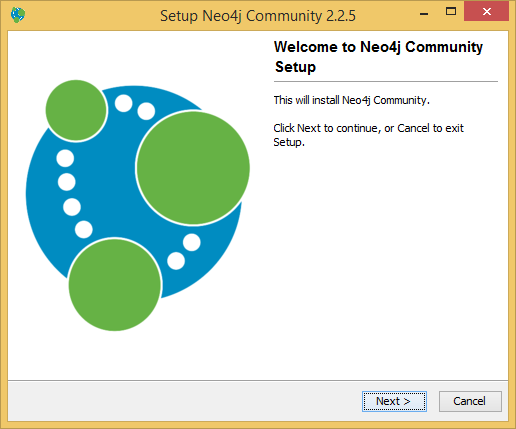
\includegraphics[scale=0.4]{./imagens/neo4j-install-step1.png}}
	\caption[Tela de boas vindas da instalação do Neo4j]
	{Tela de boas vindas da instalação do Neo4j. \textbf{Fonte:} Elaborado pelos autores.}
	\label{fig:boas_vindas_neo4j}
\end{figure}

\par A próxima tela apresentada ao usuário diz respeito ao contrato de uso do \textit{software}, como mostra a Figura~\ref{fig:contrato_neo4j}. Após lê-lo, deve-se aceitar os termos do contrato e clicar em \textit{Next}.

\newpage
\begin{figure}[h!]
	\centerline{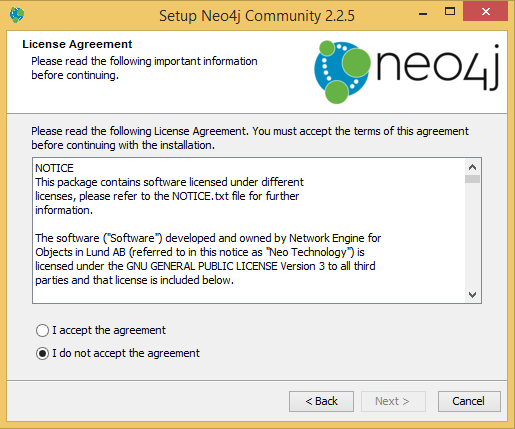
\includegraphics[scale=0.4]{./imagens/neo4j-install-step2.png}}
	\caption[Tela do contrato de uso do Neo4j]
	{Tela do contrato de uso do Neo4j. \textbf{Fonte:} Elaborado pelos autores.}
	\label{fig:contrato_neo4j}
\end{figure}

\par Na próxima tela, conforme a Figura~\ref{fig:definicao_diretorio_neo4j} demonstra, é definido o diretório de instalação do Neo4j. Por padrão este diretório é o mesmo das demais aplicações no \textit{Windows}, podendo ser alterado conforme a necessidade. Após definir o diretório de instalação deve-se clicar no botão \textit{Next}.

\begin{figure}[h!]
	\centerline{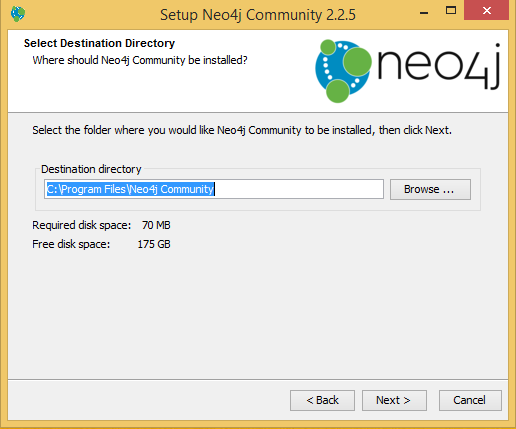
\includegraphics[scale=0.4]{./imagens/neo4j-install-step3.png}}
	\caption[Tela para definição do diretório de instalação do Neo4j]
	{Tela para definição do diretório de instalação do Neo4j. \textbf{Fonte:} Elaborado pelos autores.}
	\label{fig:definicao_diretorio_neo4j}
\end{figure}

\par Após as definições anteriores, uma tela é apresentada questionando o usuário a respeito da criação de atalhos na área de trabalho, como é demonstrado na Figura~\ref{fig:criacao_atalho_neo4j}. Posterior à definição dos atalhos do Neo4j, deve-se clicar no botão \textit{Next}.

\begin{figure}[h!]
	\centerline{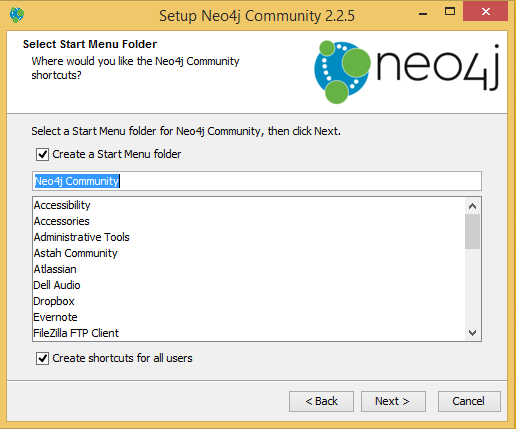
\includegraphics[scale=0.4]{./imagens/neo4j-install-step4.png}}
	\caption[Tela para criação de atalhos do Neo4j]
	{Tela para criação de atalhos do Neo4j. \textbf{Fonte:} Elaborado pelos autores.}
	\label{fig:criacao_atalho_neo4j}
\end{figure}

\par Após realizar os procedimentos descritos para a instalação do Neo4j a tela final de instalação será apresentada, informando-o a respeito do resultado da instalação conforme demonstra a Figura~\ref{fig:tela_final_neo4j}. Clique no botão \textit{Finish} para finalizar o processo de instalação.
Após todos os passos realizados com sucesso, o Neo4j estará disponível.

\begin{figure}[h!]
	\centerline{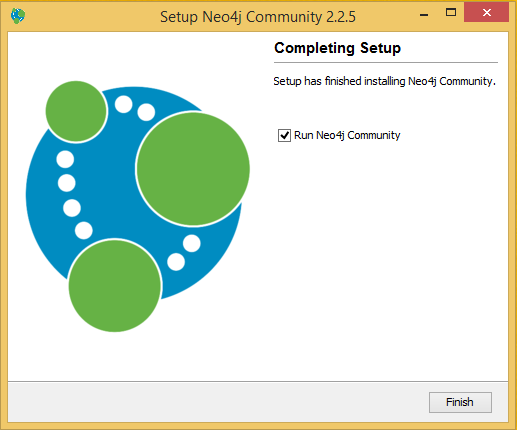
\includegraphics[scale=0.4]{./imagens/neo4j-install-step5.png}}
	\caption[Tela final de instalação do Neo4j]
	{Tela final de instalação do Neo4j. \textbf{Fonte:} Elaborado pelos autores.}
	\label{fig:tela_final_neo4j}
	
\end{figure}

\par A Figura~\ref{fig:tela_inicial_neo4j} e~\ref{fig:exemplo_consulta_neo4j} apresentam a tela inicial do banco de dados Neo4j e um exemplo de consulta realizada por meio da aplicação de gerência da base de dados.

\begin{figure}[h!]
	\centerline{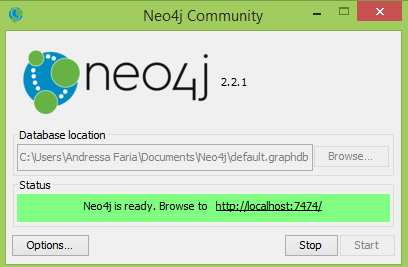
\includegraphics[scale=0.60]{./imagens/neo4j.jpg}}
	\caption[Tela de inicialização do Neo4j ]
	{Tela de inicialização do Neo4j \textbf{Fonte:} Elaborado pelos autores.}
	\label{fig:tela_inicial_neo4j}
\end{figure}

\begin{figure}[h!]
	\centerline{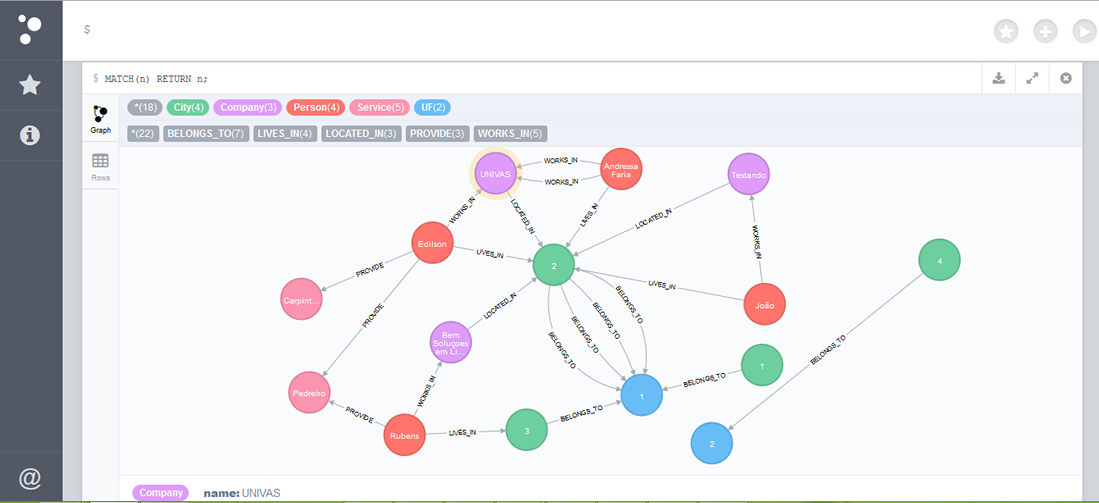
\includegraphics[scale=0.4]{./imagens/neo4j2.jpg}}
	\caption[Demonstração de uma consulta Cypher.]
	{Demonstração de uma consulta Cypher. \textbf{Fonte:} Elaborado pelos autores.}
	\label{fig:exemplo_consulta_neo4j}
\end{figure}